\documentclass[11pt,a4paper]{article}

\usepackage[T1]{fontenc}
\usepackage[utf8]{inputenc}
\usepackage{amsmath}
\usepackage{microtype}
\usepackage[margin=1in]{geometry}
\usepackage{array,booktabs,tabularx}
\usepackage[dvipsnames]{xcolor}
\usepackage{tikz}
\usetikzlibrary{positioning,arrows.meta,calc,decorations.pathreplacing}
\usepackage{listings}
\usepackage[font=small,labelfont=bf]{caption}
\usepackage{enumitem}
\usepackage[colorlinks,linkcolor=MidnightBlue,urlcolor=MidnightBlue]{hyperref}
\usepackage[nameinlink]{cleveref}

\newcommand{\lang}{Mex}
\newcommand{\ext}{\texttt{.mx}}

\newcommand{\kw}[1]{\textbf{\texttt{#1}}}
\newcommand{\nt}[1]{\textit{#1}}
\newcommand{\tok}[1]{\texttt{"#1"}}
\newcommand{\hx}[1]{\texttt{0x#1}}
\newcommand{\vm}{VM16}
\newcommand{\op}[1]{\texttt{#1}}

\definecolor{codec}{HTML}{FCE8D2}
\definecolor{heapc}{HTML}{DDF0DC}
\definecolor{stackc}{HTML}{DCE9F7}

\lstdefinelanguage{mex}{morekeywords={fun,var,if,else,while,return,break,continue,nil,true,false},
  sensitive=true, morecomment=[l]{//}, morestring=[b]", morestring=[b]'}
\lstset{language=mex, basicstyle=\ttfamily\small, keywordstyle=\bfseries,
  commentstyle=\color{black!55}, columns=fullflexible, keepspaces,
  showstringspaces=false,
  frame=single, rulecolor=\color{black!30}, xleftmargin=6pt, xrightmargin=6pt,
  aboveskip=8pt, belowskip=8pt}
\lstdefinestyle{shell}{language={}, keywordstyle={}, frame=none, backgroundcolor=\color{black!4}}

\tikzset{>=Stealth, every picture/.append style={font=\small}}
\setlength{\parskip}{3pt}

\title{\lang: Scheme Without the Brackets, for \vm{}\\[4pt]
\large Specification, version 0.1 (draft)}
\author{}
\date{\today}

\begin{document}
\maketitle

\begin{abstract}
\noindent
\lang{} is a small language with the data and functions of Scheme (pairs,
symbols, first-class functions with closures, proper tail calls) and the
syntax of C (infix operators, braces, statements). It has two data
structures: the pair, from which lists and trees are built, and the hash
table, which serves as dictionary, record and array. It is designed to compile itself on \vm{},
running on a real Z80 or 6502 with 64\,KB of memory. This document defines
its syntax (in BNF), its values and their meaning, their representation on
\vm{}, and the plan for bootstrapping the compiler.
\end{abstract}

% =====================================================================
\section{Goals}

\begin{enumerate}[nosep]
\item \textbf{Self-hosting on 8-bit hardware.} The compiler is written in
  \lang{}, and it compiles itself on \vm{} within 64\,KB.
\item \textbf{A small core.} Six types of value, two data structures,
  fifteen built-in functions. What a larger language provides as a type
  (strings, arrays, records) is made from these.
\item \textbf{Simple to compile.} A one-pass recursive-descent compiler,
  with no syntax tree, emits \vm{} code directly.
\end{enumerate}
Non-goals: speed, floating point, macros, \texttt{call/cc}, and
integers wider than 15 bits.

\paragraph{Related languages.} The idea is old. McCarthy meant Lisp
programs to be written as M-expressions, with S-expressions only for data;
Logo is Lisp without the brackets; Dylan gave a Scheme-like core an infix
syntax; and JavaScript and Lua are close relatives in all but their data.
\lang{} takes the smallest possible version of the idea.

% =====================================================================
\section{A first example}

\begin{lstlisting}
// Evaluate arithmetic expressions over variables.

var ops = {                     // operator -> function
    "+": fun (a, b) { return a + b; },
    "-": fun (a, b) { return a - b; },
    "*": fun (a, b) { return a * b; },
    "/": fun (a, b) { return a / b; }
};

// An expression is a table used as a record.
fun num(n)        { return {kind: "num", value: n}; }
fun ref(x)        { return {kind: "var", name: x}; }
fun bin(op, l, r) { return {kind: "op", op: op, left: l, right: r}; }

fun eval(e, env) {              // the value of e, with variables from env
    if (e.kind == "num") { return e.value; }
    if (e.kind == "var") { return env[e.name] || error("unbound variable"); }
    return ops[e.op](eval(e.left, env), eval(e.right, env));
}

fun vars(e, seen) {             // add the variables of e to the table seen
    if (e.kind == "var") { seen[e.name] = true; }
    if (e.kind == "op") { vars(e.left, seen); vars(e.right, seen); }
    return seen;
}

fun each(l, f) {                // call f on every element of the list l
    if (l == nil) { return nil; }
    f(hd(l));
    return each(tl(l), f);      // a tail call: this is a loop
}

fun main() {
    var e = bin("*", bin("+", ref("x"), num(3)),     // (x + 3) * (y - x)
                     bin("-", ref("y"), ref("x")));
    print(eval(e, {x: 4, y: 10}));                   // 42
    putc('\n');
    each(keys(vars(e, {})), fun (v) { print(v); putc(' '); });   // x y
    putc('\n');
}
\end{lstlisting}
Tables play three parts here. Each node of the expression is a
\emph{record}, a table with symbol keys read as \verb|e.kind| and
\verb|e.left|. The variables and their values are a \emph{dictionary},
\verb|{x: 4, y: 10}|, and so is \verb|seen|, used as a set. And \verb|ops|
is a \emph{dispatch table} from operator symbols to functions, so
\verb|ops[e.op](a, b)| calls the right one. \texttt{keys} lists the
variables in the order they were first stored, so the program always prints
\texttt{x y}. The list it returns is made of pairs, the other data structure,
and \verb|each| walks it with a tail call, which runs in constant space.

A program is a series of global variable and function definitions. Running
it first defines every function, then initialises the global variables in
order, and then calls \texttt{main()}.

% =====================================================================
\section{Lexical structure}

\begin{center}
\small
\begin{tabularx}{\linewidth}{@{}l X@{}}
\toprule
token & form\\
\midrule
name & a letter or \texttt{\_}, then letters, digits and \texttt{\_}\\
integer & decimal digits, or \texttt{0x} and hexadecimal digits; at most \hx{7FFF}, taken modulo $2^{15}$\\
character & \texttt{'a'}: one character or escape between single quotes; its value is an integer\\
symbol & \texttt{"text"}: characters and escapes between double quotes; its value is the symbol with that name\\
escape & \texttt{\textbackslash n \textbackslash t \textbackslash r \textbackslash 0 \textbackslash\textbackslash{} \textbackslash' \textbackslash\textquotedbl{} \textbackslash x}$hh$\\
keyword & \kw{fun var if else while return break continue nil true false}\\
operator & \texttt{( ) \{ \} [ ] , ; : .\ = == != < <= > >= + - * / \% ! \&\& ||}\\
comment & \texttt{//} to the end of the line\\
\bottomrule
\end{tabularx}
\end{center}
Spaces, tabs and newlines separate tokens and have no other meaning. Names
are case-sensitive. There is no string type: \verb|"expected ;"| is a symbol,
like \verb|"if"|, and is what an error message or a keyword table is made of.

% =====================================================================
\section{Grammar}

In the grammar, $\{\,x\,\}$ means zero or more $x$, $[\,x\,]$ means an
optional $x$, and quoted text is a token. Precedence is encoded in the
grammar, loosest first. The binary operators are left-associative, except
\tok{:}, which is right-associative (\verb|1 : 2 : nil| is
\verb|1 : (2 : nil)|), and the comparisons, which do not associate. The
whole grammar is in \cref{fig:grammar}.

\begin{figure}[t]
\centering
\renewcommand{\arraystretch}{1.15}
\begin{tabular}{@{}r@{\quad}c@{\quad}l@{}}
\nt{program}  & ::= & $\{$ \nt{global} $\}$\\
\nt{global}   & ::= & \nt{vardecl} $\mid$ \tok{fun} \textsc{name} \nt{function}\\
\nt{function} & ::= & \tok{(} [ \nt{params} ] \tok{)} \nt{block}\\
\nt{params}   & ::= & \textsc{name} $\{$ \tok{,} \textsc{name} $\}$\\
\nt{vardecl}  & ::= & \tok{var} \textsc{name} [ \tok{=} \nt{expr} ] \tok{;}\\[5pt]
\nt{block}    & ::= & \tok{\{} $\{$ \nt{stmt} $\}$ \tok{\}}\\
\nt{stmt}     & ::= & \nt{vardecl} $\mid$ \nt{block} $\mid$ \nt{if}\\
              & $\mid$ & \tok{while} \tok{(} \nt{expr} \tok{)} \nt{block}\\
              & $\mid$ & \tok{return} [ \nt{expr} ] \tok{;}
                $\;\mid\;$ \tok{break} \tok{;} $\;\mid\;$ \tok{continue} \tok{;}\\
              & $\mid$ & \nt{expr} [ \tok{=} \nt{expr} ] \tok{;}\\
\nt{if}       & ::= & \tok{if} \tok{(} \nt{expr} \tok{)} \nt{block} [ \tok{else} ( \nt{block} $\mid$ \nt{if} ) ]\\[5pt]
\nt{expr}     & ::= & \nt{and} $\{$ \tok{||} \nt{and} $\}$\\
\nt{and}      & ::= & \nt{compare} $\{$ \tok{\&\&} \nt{compare} $\}$\\
\nt{compare}  & ::= & \nt{cons} [ ( \tok{==} $\mid$ \tok{!=} $\mid$ \tok{<} $\mid$ \tok{<=} $\mid$ \tok{>} $\mid$ \tok{>=} ) \nt{cons} ]\\
\nt{cons}     & ::= & \nt{sum} [ \tok{:} \nt{cons} ]\\
\nt{sum}      & ::= & \nt{product} $\{$ ( \tok{+} $\mid$ \tok{-} ) \nt{product} $\}$\\
\nt{product}  & ::= & \nt{unary} $\{$ ( \tok{*} $\mid$ \tok{/} $\mid$ \tok{\%} ) \nt{unary} $\}$\\
\nt{unary}    & ::= & ( \tok{-} $\mid$ \tok{!} ) \nt{unary} $\mid$ \nt{postfix}\\
\nt{postfix}  & ::= & \nt{primary} $\{$ \tok{(} [ \nt{args} ] \tok{)} $\mid$ \tok{[} \nt{expr} \tok{]} $\mid$ \tok{.} \textsc{name} $\}$\\
\nt{args}     & ::= & \nt{expr} $\{$ \tok{,} \nt{expr} $\}$\\
\nt{primary}  & ::= & \textsc{name} $\mid$ \textsc{integer} $\mid$ \textsc{character} $\mid$ \textsc{symbol}
                $\mid$ \tok{nil} $\mid$ \tok{true} $\mid$ \tok{false}\\
              & $\mid$ & \tok{(} \nt{expr} \tok{)} $\mid$ \tok{[} [ \nt{args} ] \tok{]}
                $\mid$ \nt{table} $\mid$ \tok{fun} \nt{function}\\
\nt{table}    & ::= & \tok{\{} [ \nt{entry} $\{$ \tok{,} \nt{entry} $\}$ ] \tok{\}}\\
\nt{entry}    & ::= & ( \textsc{name} $\mid$ \textsc{symbol} $\mid$ \textsc{integer} $\mid$ \textsc{character} ) \tok{:} \nt{expr}\\
\end{tabular}
\caption{The grammar of \lang.}
\label{fig:grammar}
\end{figure}

\paragraph{Notes.}
\begin{itemize}[nosep]
\item Braces are required around every body, so there is no dangling
  \kw{else}.
\item The left side of \tok{=} must be a \textsc{name}, or a
  \nt{postfix} ending in \tok{[}\ldots\tok{]} or \tok{.}\textsc{name}.
  Assignment is a statement, not an expression. A pair is changed with
  \texttt{sethd} and \texttt{settl}.
\item A \nt{block} as a statement and a \nt{table} as an expression never
  meet: a statement that starts with \tok{\{} is a block.
\item In an \nt{entry}, the key is one token, so the \tok{:} after it is
  never the pair operator: in \verb|{a: 1 : nil}| the value is the list
  \verb|1 : nil|.
\item The grammar is LL(1). Whether an expression statement is an assignment
  is only known at the \tok{=}, so the compiler emits nothing for the last
  name or indexing step of an expression until it sees the next token.
\item \tok{fun} at the start of a global is a definition; anywhere in an
  expression it makes an anonymous function. A statement that starts with
  \tok{fun} is an expression statement.
\end{itemize}

% =====================================================================
\section{Values and meaning}\label{sec:values}

Every value has one of six types:

\begin{center}
\small
\begin{tabularx}{\linewidth}{@{}l X@{}}
\toprule
type & values\\
\midrule
nil & the single value \kw{nil}, which is the empty list and the only false
  value. \kw{false} is another name for it\\
integer & $-16384$ to $16383$. Arithmetic wraps modulo $2^{15}$. A character
  is its code\\
pair & a cell holding two values, its head and its tail\\
symbol & a name. Two symbols with the same name are the same symbol.
  \kw{true} is the symbol \texttt{"true"}\\
table & a hash table: a mutable map from keys to values\\
function & a function defined with \kw{fun}, with the values of the
  variables it captured, or a built-in function\\
\bottomrule
\end{tabularx}
\end{center}

\paragraph{Truth.} \kw{nil} is false; every other value is true, including
0. The comparisons and \verb|!| return \kw{true} or \kw{nil}.
\verb|a && b| is \kw{nil} if \verb|a| is, and otherwise \verb|b|;
\verb!a || b! is \verb|a| unless it is \kw{nil}, and otherwise \verb|b|.
Neither evaluates \verb|b| unless it needs to, so
\verb!lookup(k, env) || error("unbound")! is a common idiom.

\paragraph{Operators.}
\begin{itemize}[nosep]
\item \verb|+ - * / %| take integers; \verb|/| and \verb|%| truncate towards
  zero, as in C, and division by zero is an error.
\item \verb|h : t| makes a new pair with head \verb|h| and tail \verb|t|.
  \verb|[a, b, c]| is short for \verb|a : b : c : nil|.
\item \verb|< <= > >=| compare two integers, or two symbols by their names
  in byte order, which is enough to keep a binary search tree.
\item \verb|==| and \verb|!=| take any two values. Integers are equal when
  their values are; any other value, a table included, is equal only to
  itself. Because
  symbols are interned, two symbols are equal exactly when their names are.
  Whether two lists have equal elements is a function of the library.
\end{itemize}
Any other combination of operand types is a run-time error.

\paragraph{Tables.} \verb|t[k]| is the value stored under the key
\verb|k| in the table \verb|t|, or \kw{nil}. \verb|t[k] = v| stores it,
replacing any value already there, and storing \kw{nil} removes the key. Any
value but \kw{nil} can be a key, and keys are compared as by \verb|==|: an
integer by its value, a symbol by its name, a pair, function or table by
its identity. \verb|t.name| is short for \verb|t["name"]|, so a table with
symbol keys is a record. \verb|{a: 1, "b c": 2, 7: 3}| makes a new table; a
\textsc{name} before \tok{:} is a symbol key.

\texttt{keys(t)} is a new list of the keys of \verb|t| in the order they
were first stored, counting a key that was removed and stored again as new.
The order is therefore the same on every implementation and every run, which
the bootstrap test (\cref{sec:bootstrap}) depends on. Because the list is a
copy, a loop over it may change the table.

\paragraph{Variables and scope.} A \kw{var} at the top level declares a
global; one inside a function declares a local, visible from the end of its
declaration to the end of the enclosing block, so \verb|var x = x;| reads an
outer \verb|x|. Parameters are locals, in the same scope as the function's
outermost block. A name that is not a local refers to a global, which may
be declared later in the program. Every global that is used must be declared
somewhere, no name may be declared twice in the same scope, and the names of
the built-in functions cannot be declared at all.

\paragraph{Functions and closures.} Functions are values. \verb|fun (x) {...}|
in an expression makes a new function, which may use the locals of the
functions around it. It captures their \emph{values} when it is made: a
local that a function captures cannot be assigned anywhere, before or after
the capture, so the copy and the original can never differ. State that
several functions share lives in a pair, a table or a global:
\begin{lstlisting}
fun counter() {                 // a function that counts its calls
    var n = 0 : nil;            // a pair as a mutable box
    return fun () { sethd(n, hd(n) + 1); return hd(n); };
}
\end{lstlisting}
Calling a value that is not a function, or with the wrong number of
arguments, is an error. A function that ends without \kw{return} returns
\kw{nil}. Arguments are evaluated left to right, and the function itself
before them.

\paragraph{Tail calls.} In \verb|return f(...);| the call is a tail call:
it reuses the frame of the function that makes it, so a recursion in tail
position runs in constant space, as in Scheme. \verb|each| in the first
example is a loop.

\paragraph{Errors.} A run-time error prints a message and stops the program
with exit status 1. There is no way to catch an error.

% =====================================================================
\section{Built-in functions}

The built-ins are global functions with reserved names.

\begin{center}
\small
\begin{tabularx}{\linewidth}{@{}l X@{}}
\toprule
function & result\\
\midrule
\texttt{hd(p)}, \texttt{tl(p)} & the head or the tail of the pair \verb|p|\\
\texttt{sethd(p, v)}, \texttt{settl(p, v)} & stores \verb|v| as the head or the tail of \verb|p|\\
\texttt{intern(l)} & the symbol whose name is the list of character codes \verb|l|\\
\texttt{name(s)} & the name of the symbol \verb|s|, as a new list of character codes\\
\texttt{keys(t)} & the keys of the table \verb|t|, as a new list, in the order they were first stored\\
\texttt{size(t)} & the number of keys in the table \verb|t|\\
\texttt{type(v)} & \verb|"nil"|, \verb|"int"|, \verb|"pair"|, \verb|"sym"|, \verb|"table"| or \verb|"fun"|\\
\texttt{getc()} & the next byte of standard input, or $-1$ at end of input\\
\texttt{putc(c)} & writes the byte $c \bmod 256$\\
\texttt{putw(n)} & writes $n \bmod 2^{15}$ as a little-endian word\\
\texttt{print(v)} & writes an integer in decimal, or a symbol's name\\
\texttt{error(s)} & prints the symbol \verb|s| and stops with an error\\
\texttt{exit(n)} & stops with exit status \verb|n|\\
\bottomrule
\end{tabularx}
\end{center}
Everything else (\texttt{reverse}, \texttt{length}, \texttt{append},
\texttt{map}, \texttt{equal}, printing a list) is written in \lang.

% =====================================================================
\section{Pairs or tables}\label{sec:library}

The two structures cover each other's weak points.

\paragraph{Tables} are the dictionary (\verb|env[x]|), the record
(\verb|{op: "+", left: a, right: b}|, read as \verb|e.left|) and the array
(\verb|t[0]|, \verb|t[1]|, \ldots, with \texttt{size(t)} as the length).
Lookup takes constant time on average, and an entry costs a few words.

\paragraph{Pairs} are the list, and lists are \emph{persistent}: putting a
pair in front of a list leaves the list unchanged. That makes them the
natural environment for nested scopes. An association list, a list of
\verb|key : value| pairs, gains a binding in constant time, and the old
environment is simply the old list:
\begin{lstlisting}
fun assoc(k, a) {               // the pair (k : v) in a, or nil
    while (a != nil) {
        if (hd(hd(a)) == k) { return hd(a); }
        a = tl(a);
    }
    return nil;
}
\end{lstlisting}
A string is a list of character codes, built with \verb|:| and turned into
a symbol by \texttt{intern} when it has to be compared or kept.

The compiler uses both. Globals go in a table from symbol to slot. The
locals of the function being compiled are an association list from symbol to
frame offset: entering a block saves the list and leaving it restores it, so
scopes cost nothing. The code of one function is a list of bytes, newest
first, and a jump is patched by keeping the pair that holds its placeholder
and calling \texttt{sethd} on it when the target is known.

% =====================================================================
\section{Representation on \vm{}}\label{sec:repr}

This section is not part of the language; it is the plan for the first
implementation.

\paragraph{Values} are single 16-bit words, told apart by their low bits and
their address:
\begin{center}
\small
\begin{tabular}{@{}l l@{}}
\toprule
word & value\\
\midrule
$2n+1$ (odd) & the integer $n$\\
0 & \kw{nil}\\
even, below \texttt{HEAP} & a symbol: the address of its entry in the symbol area\\
$4k$, from \texttt{HEAP} up & a pair: the address of its cell\\
$4k+2$, from \texttt{HEAP} up & a function or a table: the address of its cell plus 2\\
\bottomrule
\end{tabular}
\end{center}
Integer arithmetic on tagged words is cheap ($a+b$ is $a+b-1$), as in the CAM
and the graph reducer of this repository. The type of a value is found from
the value alone, except that a function and a table are told apart by the
first word of their cell.

\paragraph{Cells.} The heap is an array of two-word cells, aligned on
4~bytes, with no header. A pair's cell holds its head and tail. A function's
cell holds the address of its code and its environment: \kw{nil}, or the list
of the values it captured, in the order the compiler numbered them. A built-in
is a function with \kw{nil} environment whose code is a runtime routine. Each
global function is one cell, made when the program starts. A table's cell
holds the address of its block (below) and \kw{nil}: a code address is
below \texttt{HEAP} and a block is above it, which is how the two are told
apart.

\paragraph{Tables} are compact hash tables, as in CPython. A table's block
holds a header (the address of its cell, the capacity $n$, the number of
entries used), an array of $n$ entries \texttt{(key, value)} in the order
they were stored, an index of $2n$ words, each 0 or an entry number
plus one, searched by linear probing, and a last word holding the size of
the block. Iteration walks the entries, which is
where the insertion order of \texttt{keys} comes from. Removing a key sets
its entry's value to \kw{nil} and leaves the key as a tombstone. When the
entries are used up, the table moves to a new block of twice the capacity,
or the same capacity if many entries were removed, copying only the live
entries. The hash of an integer is its value, that of a symbol is computed
from its name when it is interned and kept in its entry, and that of a pair,
function or table is its address, which is fixed because cells never
move. A new table has capacity 4, which costs 40 bytes: 6 of header, 16 of
entries, 16 of index and 2 of size.

\paragraph{Symbols} are kept in a symbol area below \texttt{HEAP}, which grows
as symbols are interned and is never collected. An entry holds a link for the
hash chain, the hash, the length and the bytes of the name. The
symbols the runtime itself needs (\verb|"true"|, the names \texttt{type}
returns) are interned first, in a fixed order, so the compiler knows their
addresses.

\paragraph{The heap} holds cells, which are allocated from its bottom up,
and table blocks, which are allocated from its top down. Cells never move;
blocks do.

\paragraph{Garbage collection} runs when the two meet. It marks, sweeps the
cells and compacts the blocks.
\begin{itemize}[nosep]
\item \emph{Mark.} The roots are the data stack and the global table. The
  mark bits are a bitmap outside the heap, one bit per cell. Marking a table
  marks its cell and then the keys and values in its block. The marker
  keeps the objects still to scan on a small stack of fixed size, outside
  the heap. If the stack overflows, the marker notes it and, once the stack
  is empty, rescans the heap for marked objects that refer to unmarked
  ones, so a deep list costs time, not space.
\item \emph{Sweep.} Every cell has the same size, so the sweep links the
  unmarked cells into a free list, and the cells never fragment.
\item \emph{Compact.} Each block starts with the address of its cell and
  ends with its size, so the blocks can be walked from the top down. A
  block whose cell is marked and still
  points to it is slid up against the last one kept, and its cell is
  updated. Every other block (a dead table's, or one its table has moved out
  of) is dropped.
\end{itemize}
A function's first word is a code address, which the collector skips.

\paragraph{Frames.} Arguments are pushed on the data stack left to right,
then the function, and \op{CALL} pushes the return address on the return
stack. The callee saves the frame pointer, pushes \kw{nil} for each local,
and addresses parameters and locals as \texttt{[fp$\pm$k]}; a captured value
$i$ is element $i$ of the environment list, which the function finds in its
own cell. A tail call copies its arguments and function over the caller's,
restores the caller's frame pointer and jumps, so the return stack does not
grow.

\paragraph{Code.} The compiler generates code for a stack machine on
\vm{}'s data stack, with integer operations inline after a test of the low
bits, and calls runtime routines for allocation, calls through values and
comparisons of symbols.

\begin{figure}[t]
\centering
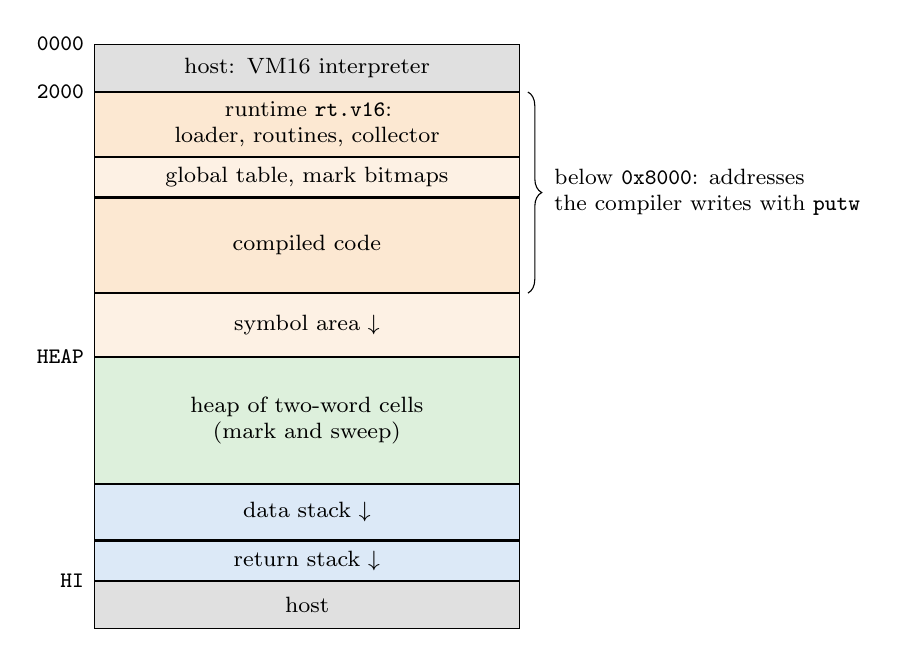
\begin{tikzpicture}[
  mem/.style={draw, text width=5.2cm, inner xsep=0.1cm, align=center, font=\footnotesize},
  adr/.style={font=\footnotesize\ttfamily, anchor=east}]
\node[mem, fill=black!12, minimum height=0.6cm] (m0) {host: \vm{} interpreter};
\node[mem, fill=codec, minimum height=0.8cm, below=0pt of m0] (m1) {runtime \texttt{rt.v16}:\\loader, routines, collector};
\node[mem, fill=codec!60, minimum height=0.5cm, below=0pt of m1] (m2) {global table, mark bitmaps};
\node[mem, fill=codec, minimum height=1.2cm, below=0pt of m2] (m3) {compiled code};
\node[mem, fill=codec!60, minimum height=0.8cm, below=0pt of m3] (m3b) {symbol area $\downarrow$};
\node[mem, fill=heapc, minimum height=1.6cm, below=0pt of m3b] (m4) {heap of two-word cells\\(mark and sweep)};
\node[mem, fill=stackc, minimum height=0.7cm, below=0pt of m4] (m5) {data stack $\downarrow$};
\node[mem, fill=stackc, minimum height=0.5cm, below=0pt of m5] (m6) {return stack $\downarrow$};
\node[mem, fill=black!12, minimum height=0.6cm, below=0pt of m6] (m7) {host};
\node[adr] at (m0.north west) {0000};
\node[adr] at (m1.north west) {2000};
\node[adr] at (m4.north west) {HEAP};
\node[adr] at (m7.north west) {HI};
\draw[decorate, decoration={brace, amplitude=5pt}] ($(m1.north east)+(0.1,0)$) --
  node[right=6pt, align=left, font=\footnotesize] {below \hx{8000}: addresses\\the compiler writes with \texttt{putw}} ($(m3.south east)+(0.1,0)$);
\end{tikzpicture}
\caption{The planned memory map. \texttt{HEAP} is fixed when the runtime is
assembled; with the heap from \hx{8000} to \hx{E000}, it holds 6144 cells.}
\label{fig:memory}
\end{figure}

% =====================================================================
\section{Programs and the compiler}\label{sec:compiler}

\paragraph{The object file.} As for the graph reducer, the runtime
\texttt{rt.v16} is the image: it reads the compiled program from the start
of standard input, places it in memory and runs it, and the rest of standard
input is the program's own:
\begin{lstlisting}[style=shell]
cat prog.mxo input.txt | vm16 rt.v16
\end{lstlisting}
An object file (\texttt{.mxo}) is a sequence of chunks, each a kind byte, a
length word and that many bytes:
\begin{center}
\small
\begin{tabular}{@{}l l@{}}
\toprule
kind & meaning\\
\midrule
\texttt{C} & code: copied to the next free address of the code area\\
\texttt{Y} & a symbol literal: interned, at the next address of the symbol area\\
\texttt{E} & the end; the body is the entry address, the initialisation code\\
\bottomrule
\end{tabular}
\end{center}
The compiler writes each distinct symbol literal once, the first time it is
used, and keeps the same running addresses as the loader, so it knows where
every chunk lands.

\paragraph{The compiler} reads the source once, with one token of lookahead,
and has no syntax tree.
\begin{itemize}[nosep]
\item The code of one function is collected in a list of bytes, newest
  first, and written as a \texttt{C} chunk when the function ends
  (\cref{sec:library}).
\item An anonymous function is compiled into a buffer of its own, nested
  inside its parent's. When it ends, the compiler knows which outer locals
  it used, numbered in order of first use, and emits code in the parent to
  push their values, build the environment list and make the cell. A local
  used two levels down is captured by the function in between as well.
\item A local that has been captured is marked, and so is a local that has
  been assigned; a local with both marks is an error.
\item A call in \verb|return|'s expression is compiled as a tail call when
  it is the last thing the expression does.
\item The stores of every global function into its slot and the initialisers
  of the global variables, in program order, are collected and written at
  the end, followed by a call to \texttt{main} and a halt: the \texttt{E}
  chunk.
\end{itemize}

% =====================================================================
\section{Bootstrapping}\label{sec:bootstrap}

\begin{enumerate}[nosep]
\item Write \texttt{rt.asm}, the runtime, in \vm{} assembly, and
  \texttt{mxc.py}, a compiler from \lang{} to object files, in Python. It is
  the reference, and is written in the style of \lang{} (one pass, no syntax
  tree, only the values of \lang), so that it can be translated by hand
  almost line by line.
\item Write \texttt{mxc.mx}, the same compiler in \lang{}, and test both on
  the same programs. Their output must be identical, byte for byte.
\item Compile \texttt{mxc.mx} with \texttt{mxc.py}, giving
  \texttt{mxc1.mxo}, and use that to compile \texttt{mxc.mx} again:
\begin{lstlisting}[style=shell]
python3 mxc.py mxc.mx -o mxc1.mxo
cat mxc1.mxo mxc.mx | vm16 rt.v16 > mxc2.mxo
cmp mxc1.mxo mxc2.mxo
\end{lstlisting}
  The two files must be identical: the compiler has reached a fixpoint.
\item Repeat the last step on the Z80 build of \vm{}.
\end{enumerate}

% =====================================================================
\section{Open questions}

\begin{itemize}[nosep]
\item \textbf{Will it fit?} The heap is 24\,KB: 6144 cells, less what the
  tables take. The compiler holds one function's code at a time, at a cell
  (4~bytes) per byte of code, its global table, and the symbols, which are
  compact. The first measurement should be the peak heap
  use of the compiler compiling itself, under \texttt{mxc.py} and
  \texttt{vm16 -c}.
\item \textbf{Arrays.} A table with keys $0, 1, \ldots$ is an array, at
  about three words an element where a real array would need one. Boot's
  design gives a table a separate array part for these keys; it would cost
  a little more code in the runtime.
\item \textbf{The capture rule} (a captured local is never assigned) keeps
  closures flat and locals on the stack, at the price of an occasional
  explicit box. Scheme's rule, shared mutable variables, would need
  environments on the heap.
\item \textbf{15-bit integers} make addresses from \hx{4000} up negative;
  the compiler should compare offsets, not addresses.
\item \textbf{Strings as symbols.} Every symbol literal and every interned
  name stays in the symbol area for good. A compiler that builds many
  temporary names would fill it; one that interns only identifiers and
  messages should not.
\end{itemize}

\end{document}
